\documentclass[11pt]{article}

\usepackage[margin=2cm]{geometry}
\usepackage[table]{xcolor}
\usepackage{float}
\usepackage{tikz}
\usepackage{algorithm}
\usepackage{algpseudocode}

\usepackage[colorlinks, linkcolor=accent, urlcolor=accent]{hyperref}

\definecolor{accent}{HTML}{1F5FA8}
\colorlet{headcolor}{accent!25}
\colorlet{rowshade}{accent!6}

\makeatletter
\renewcommand\section{\@startsection{section}{1}{\z@}%
  {-3.5ex \@plus -1ex \@minus -.2ex}{2.3ex \@plus .2ex}%
  {\normalfont\Large\bfseries\color{accent}}}
\renewcommand\subsection{\@startsection{subsection}{2}{\z@}%
  {-3.25ex \@plus -1ex \@minus -.2ex}{1.5ex \@plus .2ex}%
  {\normalfont\large\bfseries\color{accent}}}
\makeatother

\colorlet{carA}{red!55}
\colorlet{carB}{accent!50}
\colorlet{lookalike}{gray!60}

\tikzset{
  >=stealth,
  box/.style={draw=#1!70!black, fill=#1!12, rounded corners=2pt,
              inner sep=4pt},
  box/.default=accent,
  road/.style={gray!30, line width=8mm},
  guess/.style={dashed, accent, thick},
  search/.style={accent, thick},
  detection/.style={green!50!black},
  rejected/.style={red},
  leader/.style={gray!70!black},
  pics/car/.style={code={
    \filldraw[fill=#1] (-0.25, -0.1) rectangle (0.25, 0.1);
  }},
  pics/car guess/.style={code={
    \draw[guess] (-0.25, -0.1) rectangle (0.25, 0.1);
  }},
}

\renewcommand{\topfraction}{0.9}
\renewcommand{\bottomfraction}{0.8}
\renewcommand{\textfraction}{0.07}
\renewcommand{\floatpagefraction}{0.8}
\setcounter{totalnumber}{4}

\title{\color{accent}\textbf{Car Detection and Tracking}\\Design Proposal}
\date{}

\begin{document}

\rowcolors{2}{rowshade}{white}

\maketitle

\begin{abstract}
All detection and tracking runs in the ground station (GCS), not on the
drone, whose computing power is unknown. It works on the received JPEG
frames, so it faces real packet loss and compression. A pretrained detector
scans every frame and finds the cars, but it has no memory and cannot tell
one car from another. An extended Kalman filter per car supplies that
memory. It predicts where each car will be, and the Hungarian method pairs
each detection with the car whose prediction it fits, inside a gate set by
the filter's own uncertainty. The matched detection then corrects the
filter. The car's ID belongs to the filter's track, so it survives lost
frames, short hiding under bridges or trees, and short trips out of view.
Cars are tracked in world metres using the drone's GPS position. The design
is scored against the simulator's true car IDs under packet loss.
\end{abstract}

\section{Goal and scope}

The assignment asks for real-time detection of moving cars in the video
stream, with a unique and persistent ID for each car. The design has four
goals:

\begin{enumerate}
  \item Find every car in every received frame, even when tens of cars are
        in view, close together and looking alike.
  \item Give each car its own ID and keep it through lost frames, JPEG
        blur, short hiding under bridges or trees, and short trips out of
        view.
  \item Follow any car motion: turning, braking, stopping and queueing.
  \item Work on a real drone with only the frame source and the
        pixels-to-metres step changed.
\end{enumerate}

\section{Architecture}

The model and the tracker run in the GCS on the received JPEG frames, with
the simulator and with a real drone. The drone only flies and streams video.
Its computing power is unknown: it may have no spare processor, or one too
weak for a model at 30 frames per second. Ground computing is cheap and can
run a bigger model, and the model can be updated without touching the
aircraft. The cost is that the GCS works on compressed frames that arrive
late and sometimes not at all, so the tracker must handle that
(Section~\ref{sec:tracker}).

\begin{figure}[htbp]
\centering
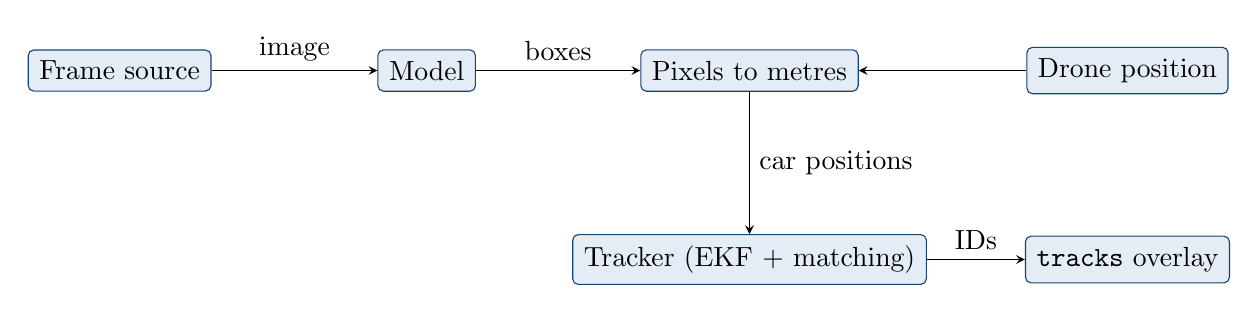
\begin{tikzpicture}
  \node[box] (source) at (0, 0) {Frame source};
  \node[box] (detect) at (3.9, 0) {Model};
  \node[box] (project) at (8, 0) {Pixels to metres};
  \node[box] (pose) at (12.8, 0) {Drone position};
  \node[box] (track) at (8, -2.4) {Tracker (EKF + matching)};
  \node[box] (ui) at (12.8, -2.4) {\texttt{tracks} overlay};

  \draw[->] (source) -- node[above] {image} (detect);
  \draw[->] (detect) -- node[above] {boxes} (project);
  \draw[->] (pose) -- (project);
  \draw[->] (project) -- node[right] {car positions} (track);
  \draw[->] (track) -- node[above] {IDs} (ui);
\end{tikzpicture}
\caption{Pipeline in the GCS.}
\end{figure}

\subsection{Where the work runs}
\label{sec:worker}

The GCS interface runs one loop that reads the sockets every few
milliseconds and redraws the screen. Detection in that loop would freeze the
video whenever a frame took long, so a separate worker does detection and
tracking. The worker has a mailbox with room for one frame, and a new frame
replaces an unread one, so a slow worker skips frames instead of falling
behind. The tracker uses the real time between the frames it sees, so a
skipped frame is handled like a lost one. Boxes and IDs are drawn as a new
\texttt{tracks} overlay, next to the existing \texttt{crosshair}. The GCS
logs how old each frame is when it arrives and how long the worker takes,
which shows whether the design keeps up on a given machine.

\subsection{Drone position}

The tracker keeps cars in world metres, so it needs the drone's position for
every frame. Telemetry carries the drone's GPS fix, or ``no fix''. The GCS
turns each fix into metres north and east of the first fix; over a few
kilometres the Earth is flat enough for this. Telemetry arrives 10 times per
second and frames 30 times per second, so the GCS interpolates between the
two nearest fixes using the simulator clock both streams carry.

Without a fix, the GCS compares each frame with the one before. Roads and
buildings all shift together when the drone moves, and that shift is the
drone's own movement. Small errors add up, so world positions slowly drift,
but the IDs of cars in view are not affected. Real GPS can jump a few
metres, so a real drone does not use the raw fix. It finds its estimated
position using a weighted mean of GPS and IMU, usually with a Kalman filter,
and the GCS uses that estimate.

\subsection{Pixels to metres}

In the simulator the camera looks straight down and the drone is always in
the centre of the image. A car's position in the world is the drone's
position plus the car's offset from the image centre, divided by 10 (10 px
per metre).

\begin{figure}[htbp]
\centering
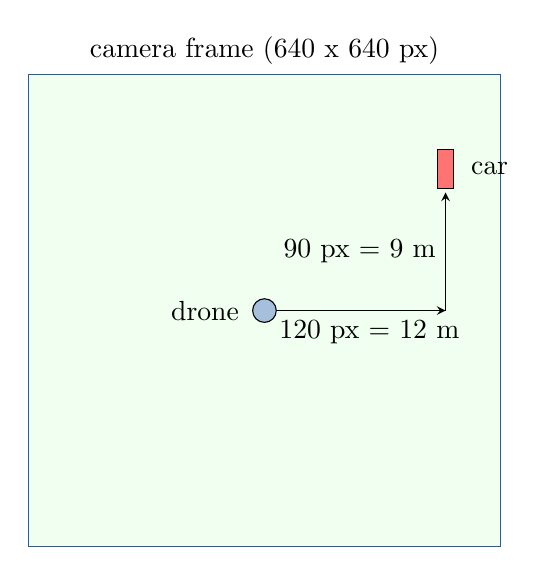
\begin{tikzpicture}
  \coordinate (drone) at (3, 3);
  \coordinate (car) at (5.3, 4.8);
  \coordinate (corner) at (car |- drone);

  \draw[accent, fill=green!6] (0, 0) rectangle (6, 6);
  \node[above] at (3, 6) {camera frame (640 x 640 px)};

  \filldraw[fill=accent!40] (drone) circle (0.15);
  \node[left=2mm] at (drone) {drone};
  \pic[rotate=90] at (car) {car=carA};
  \node[right=2mm] at (car) {car};

  \draw[->] ([xshift=1.5mm]drone) -- node[below, pos=0.55] {120 px = 12 m}
    (corner);
  \draw[->] (corner) -- node[left] {90 px = 9 m} ([yshift=-3mm]car);
\end{tikzpicture}
\caption{Pixels to metres.}
\end{figure}

On a real drone the camera may be tilted and the drone's height changes. The
same step then uses the camera's lens data, the height and the camera angle to
find where each box touches the ground. The tracker does not change.

\section{The model and the Kalman filter work together}
\label{sec:loop}

The two parts have different jobs. The model sees. It looks at one frame and
says ``there are cars here, here and here''. It is a simple model with no
memory and no sense of motion, so it cannot tell which car is which. With
the model alone, every frame would be a fresh set of boxes, and IDs would
jump between cars whenever two came close.

The Kalman filter estimates each car's position and velocity, and before
each frame it predicts where every car should be and how sure it is. It
never looks at the picture.

Together they form a loop (Figure~\ref{fig:loop}). The filter predicts every
car's position. The model scans the whole frame and returns boxes. Each box
is matched to the car whose prediction it fits
(Section~\ref{sec:matching}), and the matched box becomes that car's
measurement, which corrects the filter. The ID belongs to the filter's
track, not to the box, so a car keeps its ID as long as its boxes keep
landing where the filter expects it.

\begin{figure}[htbp]
\centering
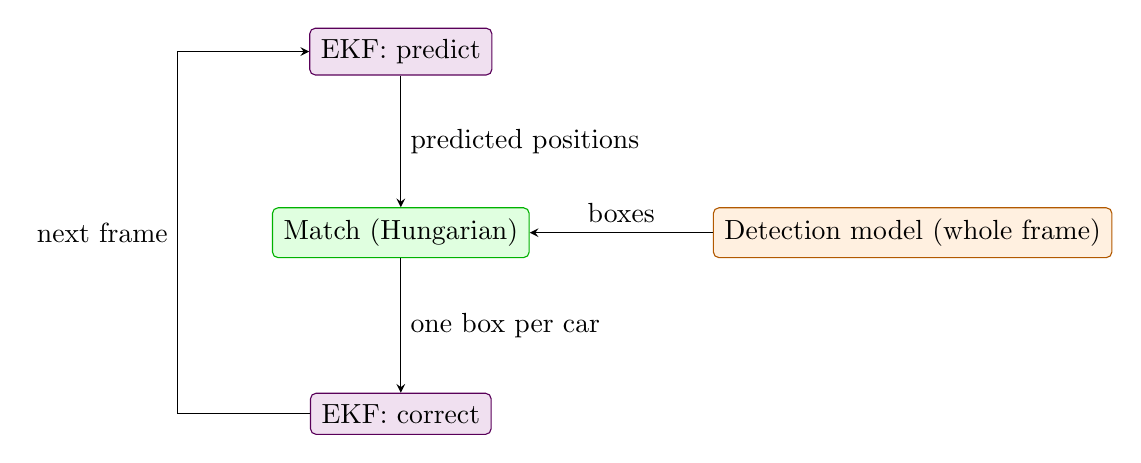
\begin{tikzpicture}
  \node[box=violet] (predict) at (0, 0) {EKF: predict};
  \node[box=green] (match) at (0, -2.3) {Match (Hungarian)};
  \node[box=violet] (correct) at (0, -4.6) {EKF: correct};
  \node[box=orange] (model) at (6.5, -2.3) {Detection model (whole frame)};
  \coordinate (back) at ([xshift=-1.2cm]match.west);

  \draw[->] (predict) -- node[right] {predicted positions} (match);
  \draw[->] (match) -- node[right] {one box per car} (correct);
  \draw[->] (model) -- node[above] {boxes} (match);
  \draw[->] (correct.west) -| (back) |- (predict.west);
  \node[left] at (back) {next frame};
\end{tikzpicture}
\caption{Detection and tracking loop.}
\label{fig:loop}
\end{figure}

\section{Detection model}

Cars are assumed to look real from above: many models and colours, windows,
roofs and shadows (in the simulator, detailed top-down sprites). A colour
rule cannot handle that, so the detector is a learned model. It sits behind
a small interface, an image in and car boxes with a confidence out, so the
model can be swapped.

\subsection{Model choice}

Training from scratch is too much work, so the detector is an existing
pretrained model, run with ONNX Runtime.

\begin{center}
\begin{tabular}{|l|l|l|}
  \hline
  \rowcolor{headcolor}
  Model & Code licence & Notes \\
  \hline
  YOLOX-Nano / Tiny & Apache-2.0 & small, easy to export \\
  NanoDet-Plus & Apache-2.0 & made for small devices \\
  RTMDet-tiny & Apache-2.0 & from OpenMMLab \\
  RT-DETR (small) & Apache-2.0 & larger, more accurate \\
  Ultralytics YOLOv8/11 & AGPL-3.0 & rejected: licence \\
  \hline
\end{tabular}
\end{center}

The proposal is YOLOX-Nano, whose code and COCO-trained weights are released
under Apache-2.0. Ultralytics models are the easiest to start with, but
Ultralytics licenses its code and every model trained with it under
AGPL-3.0, so a company must either open-source its whole project or buy an
Enterprise License. Weights may also carry the terms of the data they were
trained on. Drone-view weights are often trained on VisDrone, which is
released under CC BY-NC-SA 3.0 and so cannot be used commercially. Some
re-uploads list CC BY 4.0, but that does not change the original licence.

\subsection{What makes it hard}

Rooftop boxes, parked trailers and road markings can look like a car from
above. The model gives them a lower score, and a box that fits no car's
prediction only starts a new track, which is not shown until it has been
seen in several frames in a row (Section~\ref{sec:lifecycle}). A dark car on
a dark road, or JPEG blur, gives weak edges, and the model may miss the car
for a frame or two. The filter carries the car on its prediction until the
model finds it again.

\section{Tracker}
\label{sec:tracker}

The tracker gives every car an ID and keeps it. It follows SORT: one filter
per car, and one matching step for all cars together.

\subsection{Extended Kalman filter}

Each car's filter holds its position, speed, heading and turn rate, in world
metres. This is the constant turn rate and velocity (CTRV) model. Every
frame the filter runs the cycle of Figure~\ref{fig:loop}.

The predict step moves each car forward along its heading, bending by its
turn rate, over the real time since the last frame. After a lost frame the
step is twice as long, so the car still lands in the right place.
Predicting also makes the filter less sure, more along the direction of
travel than across it.

The correct step uses the box matched to the car
(Section~\ref{sec:matching}) as the measurement. The filter does not jump to
the box. It moves part of the way, depending on how sure it is of its
prediction compared with how noisy the detector is. A car seen steadily
trusts its prediction more, and a car just found trusts the box more. Along
the way the filter learns the car's speed, heading and turn rate.

A turning car moves along a curve, so a plain Kalman filter, which can only
model straight-line motion, does not fit. The extended Kalman filter treats
the curve as a straight line for one short step around the current
estimate. A frame lasts 33 ms, so even in a sharp turn that short step is
close to the real path. The simulated drone never rotates. A real drone
does, and the pixels-to-metres step uses its heading to turn every box into
world metres. An error in that heading moves a car's measured position,
more for cars far from the image centre, so those boxes are given more
measurement noise and the filter trusts them less.

\subsection{Gate and matching}
\label{sec:matching}

Each car's gate is the filter's own uncertainty around its predicted
position. It is an ellipse, long along the direction of travel, where speed
is least certain, and narrow across it. It is small for a car seen in the
last frame and grows each frame the car is missed. A box inside the gate may
belong to that car, and a box outside never does.

The Hungarian method then pairs boxes with cars over all cars at once. It
picks the pairing with the smallest total distance, each distance scaled by
that car's uncertainty, so two cars never take the same box. For example,
box 1 lies in both A's and B's gates, nearer B, and box 2 lies in B's gate
only. Matching each car on its own would give box 1 to B and leave A
without a box. The best total gives 1 to A and 2 to B. Tens of cars stay
cheap: gates that don't overlap split the cars into small groups, and each
group is matched on its own.

The original SORT matches by box overlap. Cars are only 2 m wide, so after
a short gap the predicted box and the new box may not overlap, and the car
would get a new ID. The gate still finds it.

The gate has a cap. Cars queued at a traffic light can be 6 m apart centre
to centre, and they often look alike. If a missed car's gate grew past half
of that, it could take the box of the car behind it, and the IDs would swap.
So the gate stops growing at about 3 m, and a car that would need more is
dropped (Section~\ref{sec:lifecycle}) instead of swapped. The cap is a
starting value that the scoring in Section~\ref{sec:testing} tunes.

\subsection{Life of a track}
\label{sec:lifecycle}

A track is in one of three states (Figure~\ref{fig:life}). A box that
matches no car starts a new track. It becomes tracked only after it is
matched in 3 frames in a row, so a one-frame look-alike never gets an ID. A
tracked car that is not matched becomes lost. It coasts on its prediction,
and its gate grows each frame. If a box lands in the gate again, the car is
tracked again with the same ID. If the gate reaches the 3 m cap first, the
track is deleted. Only tracked cars are drawn.

The same rule covers three cases. A car hidden under a bridge or a tree
usually keeps its speed, so it comes out inside its gate and keeps its ID.
A car that leaves the image coasts the same way and gets its old ID back if
it returns before the cap. A lost frame is not a miss: the tracker sees the
gap in frame numbers, predicts over the real time, and changes no state.

\begin{figure}[htbp]
\centering
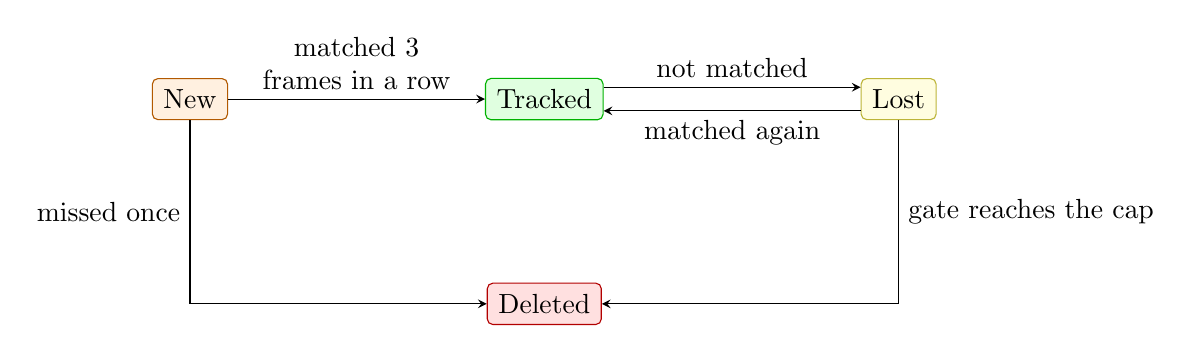
\begin{tikzpicture}
  \node[box=orange] (new) at (0, 0) {New};
  \node[box=green] (trk) at (4.5, 0) {Tracked};
  \node[box=yellow] (lost) at (9, 0) {Lost};
  \node[box=red] (del) at (4.5, -2.6) {Deleted};

  \draw[->] (new) -- node[above, align=center] {matched 3\\frames in a row}
    (trk);

  \draw[->] ([yshift=1.5mm]trk.east) -- node[above] {not matched}
    ([yshift=1.5mm]lost.west);
  \draw[->] ([yshift=-1.5mm]lost.west) -- node[below] {matched again}
    ([yshift=-1.5mm]trk.east);

  \draw[->] (new) |- node[pos=0.25, left] {missed once} (del);
  \draw[->] (lost) |- node[pos=0.25, right] {gate reaches the cap} (del);
\end{tikzpicture}
\caption{Life of a track.}
\label{fig:life}
\end{figure}

\section{Testing}
\label{sec:testing}

Unit tests feed made-up boxes into the tracker, with no network and no
images, so each hard case gives an exact, repeatable result: a turning car,
a queue, two look-alikes crossing, a car hidden or out of view. For scoring,
the simulator knows every car's true ID and, for testing only, sends it on a
debug port. The GCS compares its tracks with it and counts ID switches,
missed cars and false cars. The live test flies a fixed route over busy
roads under \texttt{tc netem} packet loss, with FEC on and off, and checks
that the scores hold. A real drone has no ground truth, so scoring there
uses recorded flights labelled by hand.

\section{Tradeoffs}

\begin{table}[H]
\centering
\small
\begin{tabular}{|>{\raggedright\arraybackslash}p{3cm}|%
  >{\raggedright\arraybackslash}p{4.6cm}|%
  >{\raggedright\arraybackslash}p{8.6cm}|}
  \hline
  \rowcolor{headcolor}
  Decision & Chosen & Reason, and what was rejected \\
  \hline
  Where it runs & GCS, on JPEG & The drone's computing power is unknown.
    Ground computing is cheap, runs a bigger model, and updates without touching
    the aircraft. Onboard: less delay and survives link drops, but needs an
    extra computer and a smaller model. \\
  Detector & Pretrained YOLOX-Nano, Apache-2.0 & Handles real-looking cars.
    From scratch: too much work. Colour rules: fail on real cars. Ultralytics
    (AGPL) and VisDrone-trained (non-commercial) weights: licence risk. \\
  Detection area & Whole frame, every frame & Simple, and a new car can't be
    missed outside a search area. Crops around predictions: less work, but more
    rules and a blind spot. \\
  Motion model & EKF, constant turn rate (CTRV) & Follows turning cars. Plain
    Kalman (straight line): drifts off in turns. IMM: handles every motion, but
    is the most complex. \\
  Matching & Hungarian, all cars together, in metres & Each box goes to one
    car only. Greedy, per car: two cars can claim one box. Box overlap (IoU):
    fails after short gaps, because cars are only 2 m wide. \\
  Gate & Filter's uncertainty ellipse, capped at 3 m & Grows with doubt and is
    shaped by direction. Fixed circle: ignores speed and direction. No cap:
    close look-alikes swap IDs. \\
  Life cycle & New, tracked, lost; deleted at the cap & One rule for hidden,
    out-of-view and missed cars. A time limit per case: more rules to tune. \\
  Appearance & None & Position is enough at 30 frames per second. DeepSORT:
    the upgrade if look-alikes swap after long gaps. \\
  \hline
\end{tabular}
\end{table}

\end{document}
